\chapter{Введение}
\label{ch:1}

According to Ginzburg-Landau theory, a conventional superconductor near 
\( T \) c is described by a single complex order parameter field. The physics 
of these systems is governed by two fundamental length scales, the magnetic
field penetration depth \( \lambda \) and the coherence length \( \xi \), and
the ratio \( \kappa \) of these determines the response to an external
field, sorting them into two categories as follows; type-I when 
\( \kappa < 1/\sqrt{2} \) and type-II when \( \kappa > 1/\sqrt{2} \)
\footnotemark[3].

Type-I superconductors expel weak magnetic fields, while strong fields give 
rise to formation of macroscopic normal domains with magnetic flux 4. The 
response of type-II superconductors is completely different; below some 
critical value \( H_{c1} \), the field is expelled. Above this value a 
superconductor forms a lattice or a liquid of vortices that have a 
supercurrent circulating around a normal core and carry magnetic flux through 
the system. Finally, at a higher second critical value, \( H_{c2} \) 
superconductivity is destroyed. 

These different responses are usually viewed as consequences of the vortex 
interaction in these systems, the energy cost of a boundary between 
superconducting and normal states and the thermodynamic stability of vortex 
excitations. In a type-II superconductor the energy cost of a boundary between 
the normal and the superconducting state is negative, while the interaction 
between vortices is repulsive 3. This leads to a formation of stable vortex 
lattices and liquids. In type-I superconductors the situation is the opposite; 
the vortex interaction is attractive (thus making them unstable against 
collapse into one large vortex), while the boundary energy between normal and 
superconducting states is positive. From a thermodynamic point of view the 
principal difference between type-I and type-II states is the following: (i) 
In type-II superconductors the external magnetic field strength required to 
make formation of vortex excitations energetically preferred, \( H_{c1} \), 
is smaller than the thermodynamical magnetic field \( H_{ct} \) (the field 
whose energy density is equal to the condensation energy of a superconductor, 
i.e. the field at which the uniform superconducting state becomes 
thermodynamically unstable); (ii) In type-I superconductors the field strength 
required to create a vortex excitation is larger than the thermodynamical 
critical magnetic field i.e. vortices cannot form. One can distinguish also a 
special "zero measure" boundary case where \( \kappa \) has a critical value 
exactly at the type-I/type-II boundary, which in the most common GL model 
parameterization corresponds to \( \kappa = 1/\sqrt{2} \). In that case 
vortices do not interact 5 in the Ginzburg-Landau theory. 

The above circumstances result in a situation where, in a strong external 
magnetic field, type-I superconductors usually have a tendency to minimize 
boundary energy between the normal and superconducting states, leading to a 
formation of large inclusions of normal phase which frequently have laminar 
structure \( ^4 \). 

Recently there has been increased interest in superconductors with several 
superconducting components. The main situations where multiple superconducting 
components arise are (i) multiband superconductors 6 - 11 , (ii) mixtures of 
independently conserved condensates such as the projected superconductivity 
in metallic hydrogen and hydrogen rich alloys 12–14 and (iii) superconductors 
with other than s-wave pairing symmetries. In this work we focus on the cases 
(i) and (ii). The principal difference between the cases (i) and (ii) is the 
absence of the inter-component Josephson coupling in case (ii). 

In two-band superconductors (i) the superconducting components originate from 
electronic Cooper pairing in different bands 6. Therefore these condensates 
could not a priori be expected to be independently conserved. This, at the 
level of effective models should manifest itself in a rather generic presence 
of intercomponent Josephson coupling. 

In the case (ii) two superconducting components were predicted to originate 
from electronic and protonic Cooper pairing in metallic hydrogen or 
hydrogen-rich alloys. In the projected liquid metallic deuteriumor 
deuterium-rich alloys, electronic superconductivity was predicted to coexist 
at ultra high pressures with deuteronic condensation 12–14 . Because electrons 
cannot be converted to protons or deuterons the condensates are independently 
conserved, and therefore in the effective model intercomponent Josephson 
coupling is forbidden on symmetry grounds. These states are currently a 
subject of a renewed experimental pursuit. They are expected to arise at high 
but experimentally accessible pressures (\( \approx 400 \)~GPa). Current 
static compression experiments achieve pressures of \( \approx 350 \)~GPa 
with pressures of an order of 1TPa being anticipated in diamond anvil cell 
experiments due to the recent availability of ultra hard diamonds. Similar 
two-charged component models were discussed in the context of the physics of 
neutron stars where they represent coexistent protonic and 
\( \Sigma^\text{--} \)-hyperon Cooper pairs in the neutron star 
interior\( ^{15} \). 

This wide variety of systems raises the need to understand and classify the 
possible magnetic responses of multicomponent superconductors. It was 
discussed recently that in multicomponent systems the magnetic response is 
much more complex than in ordinary systems, and that the type-I/type-II 
dichotomy is not sufficient for classification. Rather, in a wide range of 
parameters, as a consequence of the existence of three fundamental length 
scales, there is a separate superconducting regime where vortices have 
long-range attractive, short-range repulsive interaction and form vortex 
clusters immersed in domains of two-component Meissner state 1,2. Recent 
experimental works 16,17 have put forward the suggestion that this state is 
realized in the two-band material \( MgB_2 \), which sparked growing interest 
in this topic. In particular questions were raised over whether this 
"type-1.5" superconducting regime (as it was termed by Moshchalkov et 
al\( ^{16} \), for recent works see 18 ) is possible even in principle in the 
case of various non vanishing couplings (e.g. intrinsic Josephson coupling, 
mixed gradient couplings etc) between superconducting components in different 
bands. 

In this work we report a study of the appearance of type-1.5 superconductivity 
especially focusing on the case of multiband superconductivity, demonstrating 
the persistence of this type of superconductivity in the presence of various 
kinds of intercomponent couplings (such as interband Josephson coupling, mixed 
gradient coupling, density-density, and other kinds coupling).

\section{Сверхпроводимость типа 1,5}
\label{sec:1-1}

The possibility of a new type of superconductivity, distinct from the type-I 
and type-II in multicomponent systems 1,2 is based on the following 
considerations. In principle the boundary problem in the Ginzburg-Landau type 
of equations in the presence of phase winding is not, from a rigorous point of 
view, reducible to a one-dimensional problem in general. Furthermore, as 
discussed in 1,2 , in general in two-component models there are three 
fundamental length scales which renders the

\begin{figure}[h!]
  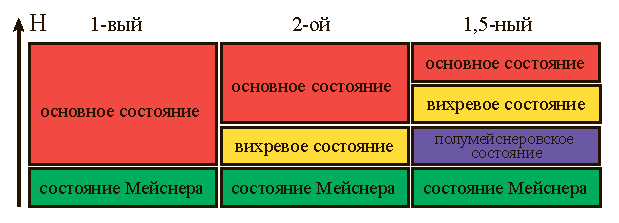
\includegraphics[width=.5\textwidth]{1-01}
  \caption{A comparison of the magnetic phase diagrams of
    clean bulk type-I,type-II and type-1.5 superconductors at
    zero temperature. The semi-Meissner state is a macroscopic
    phase separation into two-component Meissner state and vortex
    clusters where one of the density modes is suppressed by
    core overlaps}
\end{figure}


model impossible to parametrize in terms of a single dimensionless parameter 
\( \kappa \). In the case where the condensates are not coupled by interband 
Josephson coupling but only by the vector potential these length scales are
the two independent coherence lengths (set by the inverse masses of the 
corresponding scalar density fields) and magnetic field penetration length 
(set by the inverse mass acquired by the gauge field). In contrast, in the 
case where the condensates are coupled by inter-band Josephson terms, one 
cannot distinguish independent coherence lengths attributed to different 
condensates. Nonetheless, in this case the density variations can also possess 
two fundamental length scales 2 , in contrast to single-component theories. 
We elaborate on this fact below. In 1,2 vortex solutions in two-component 
theories were found which have non-monotonic vortex inter-action, with a long 
range attractive part determined by a dominant density-density interaction and 
a short range repulsive part produced by current-current and electro-magnetic 
interactions. An important circumstance which was demonstrated was that these 
vortices are thermodynamically stable in spite of the existence of the 
attractive tail in the interaction.

A non-monotonic intervortex interaction potential should result in the 
formation of vortex clusters in low magnetic field immersed into the 
vortexless areas, a state referred to in 1 as the "semi-Meissner state". 
Figure 1 shows the schematic phase diagram of a type-1.5 superconductor.

If the vortices form clusters one cannot use the usual one-dimensional 
argument concerning the energy of superconductor-to-normal state boundary to 
classify the magnetic response of the system. First of all, the energy per 
vortex in such a case depends on whether a vortex is placed in a cluster or 
not: i.e. formation of a single isolated vortex might be energetically 
unfavorable, while formation of vortex clusters is favorable, because in a 
cluster where vortices are placed in a minimum of the interaction potential, 
the energy per flux quantum issmaller than that for an isolated vortex 
(thermodynamically the nonmonotonic two-vortex interaction potential predicts 
that the smallest energy per flux quantum will be in the case of a uniform 
lattice with spacing equal to the minimum of two-body intervortex potential).

Thus, besides the energy of a vortex in a cluster, there appears an additional 
energy characteristic associated with the boundary of a cluster. In other 
words, in this situation, to determine the magnetic response of a system it is 
not sufficient to study the one-dimensional boundary problem nor the 
single-vortex problem, in contrast to single component systems. Moreover, in a 
cluster the system tends to minimize the boundary energy of a cluster 
(similarly to type-I behavior), while breaking into a lattice of one-quantum 
vortices inside the cluster (similarly to type-II systems with negative 
interface energy). Thus, in an increased magnetic field the vortices form via 
a first order phase transition. A magnetic phase distinct from the vortex and 
Meissner states which then arises is a macroscopic phase separation into 
domains of two-component Meissner state and vortex clusters where one of the 
density modes is suppressed by core overlap. We summarize the basic properties 
of type-I, type-II and type-1.5 regimes in the table I.

The existence of thermodynamically stable type-1.5 superconducting regimes 
ultimately depends on the existence of a nonmonotonic intervortex interaction 
potential. It is an important question how generic this effect is. In this 
work we mainly focus on multiband realizations of multicomponent 
superconductivity and investigate the effects of interband Josephson coupling, 
mixed gradient coupling, and density-density coupling terms on vortex 
interactions in two band superconductors. We show that (i) when these 
couplings are present, the system still can possess three fundamental length 
scales, in contrast to the two length scales in the usual single-component GL 
theory; (ii) non-monotonic interaction is possible in a wide parameter range 
in these models.

The structure of this paper is as follows: In section II we introduce the 
model.In section III we present a linear theory of asymptotics of the vortex 
fields in a superconductor with two bands with various interband couplings.

We begin section III by demonstrating that for a general form of the effective 
potential in a two-band (or more generally two-gap) Ginzburg-Landau free 
energy, the linear theory gives, under quite general conditions, two 
fundamental length scales of the variations of the densities. From the 
linearized theory we calculate the long-range intervortex interaction 
potentials using the two-component generalization of the point-vortex method 
19 and show how the non-monotonic intervortex interaction potential arise from 
the interplay of two fundamental length scales of the superfluid density 
variations and the magnetic field penetration length. The central point of 
this part is how the fundamental length scales are defined in the presence of 
interband coupling as well as the occurrence of "mode mixing". Next we move to 
quantitatively study the effects of several kinds of intercomponent couplings 
which quite generically arise in two-component theories.

In section III (d) we demonstrate that that mixed gradient coupling can lead 
under certain conditions to an increase in the disparity of the characteristic 
scales of the density variations.

In Section IV we present a large scale numerical study of the full nonlinear 
problem of the interaction between a pair of vortices.
